\documentclass{beamer}
\usepackage{ragged2e}
\usepackage{hyperref}
\usepackage{graphicx}

\title{Moters: The Material Version of toters}
\author{
  Antoine Karam\\\texttt{antoine.karam3@net.usj.edu.lb}\\[0.5cm]\and Ghady Youssef\\\texttt{ghady.youssef@net.usj.edu.lb}\\
}
\date{January 2025}

\begin{document}

\maketitle

\begin{frame}{Introduction}
    \justifying
    This application streamlines the food ordering and delivery process, allowing users to browse restaurants, place orders, and track deliveries in real time, all from a single platform. It aims to provide a convenient, efficient, and seamless experience for users, enhancing their ability to manage food orders and deliveries.
\end{frame}

\begin{frame}{Introduction}
    \begin{figure}[h]
        \centering
        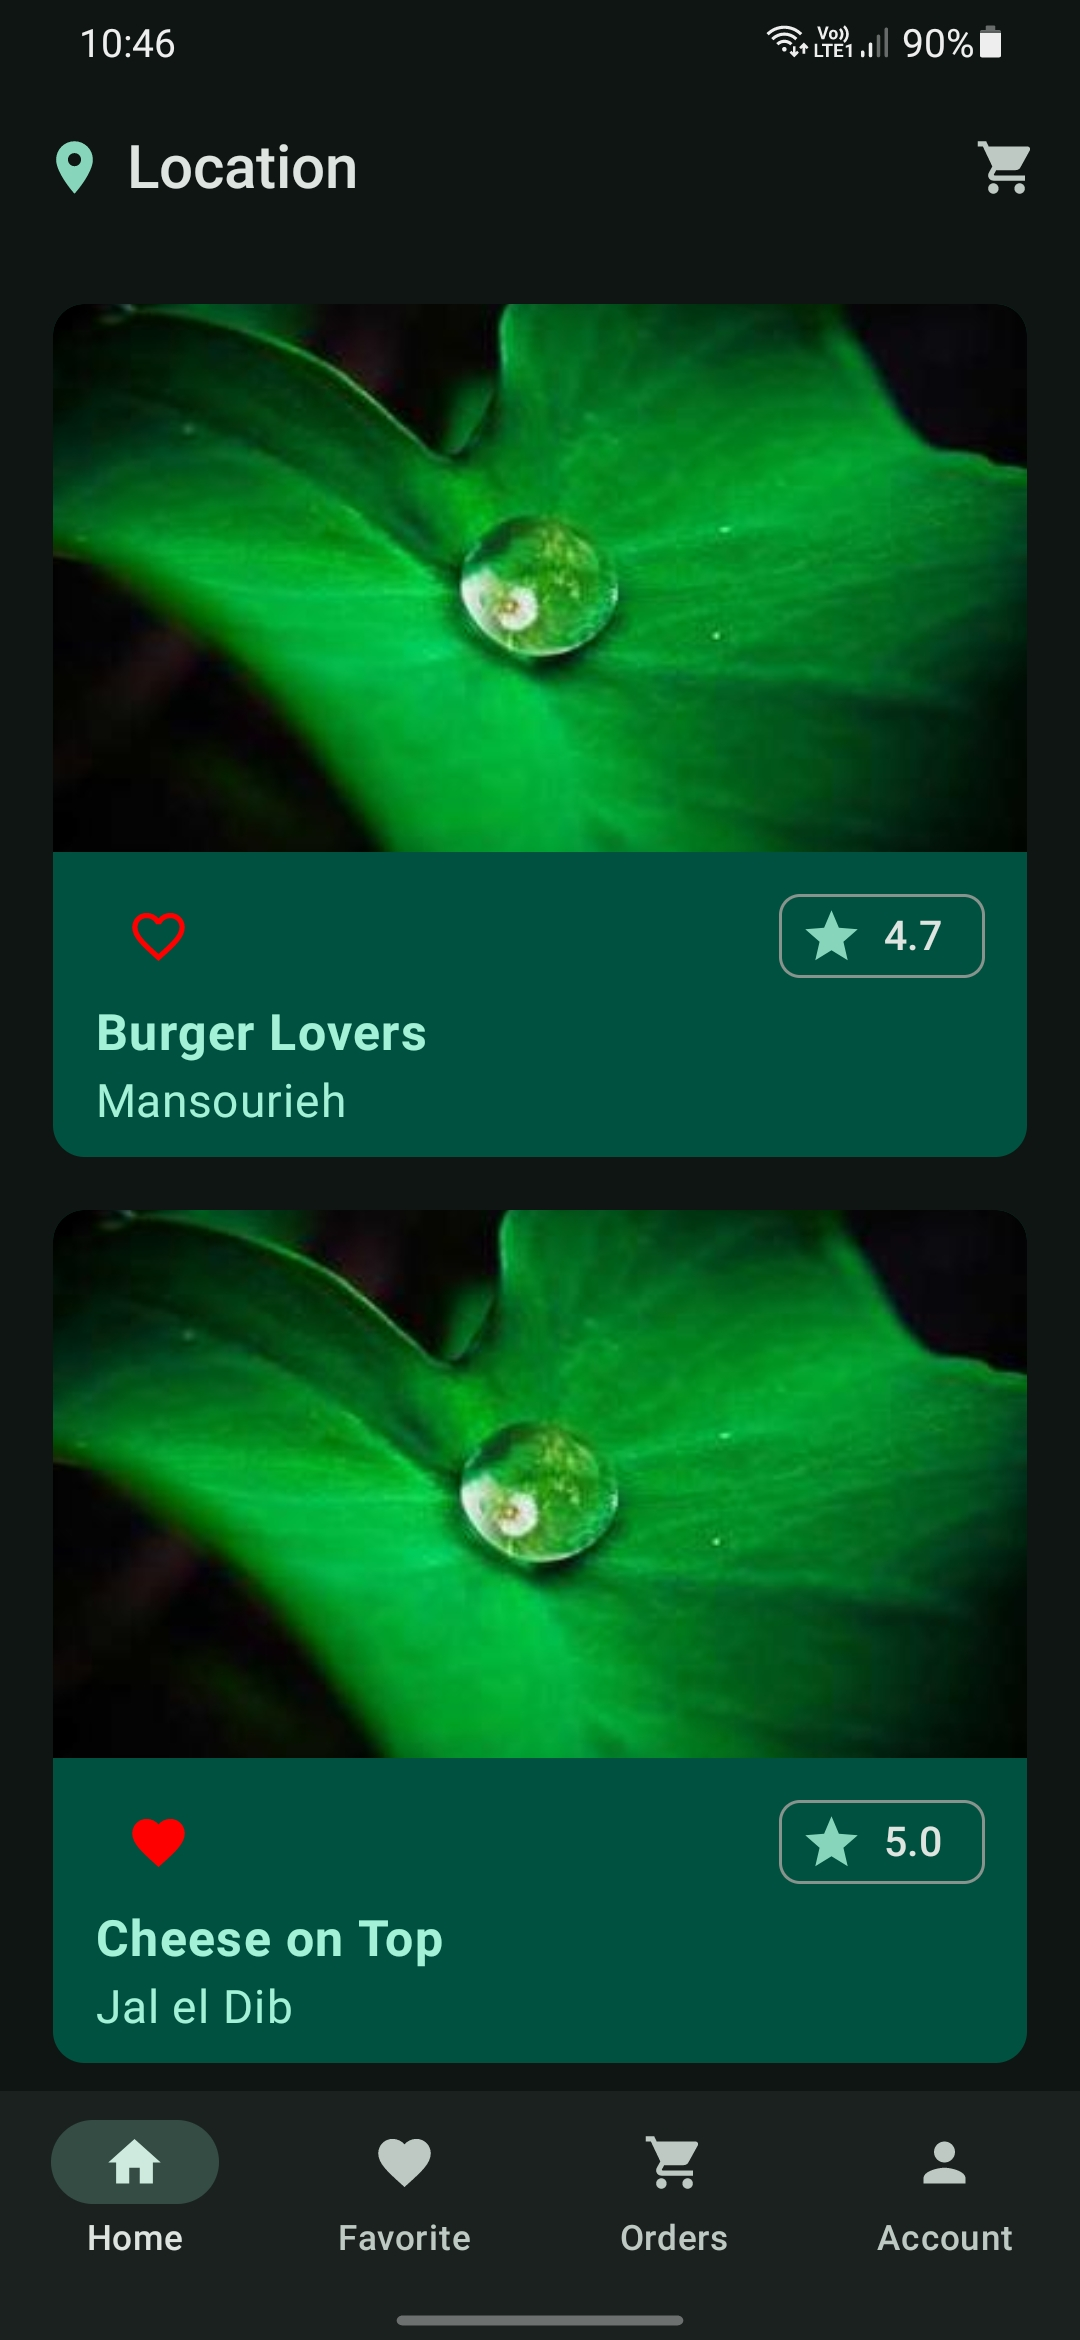
\includegraphics[height=0.7\linewidth]{assets/homepage.jpg}
        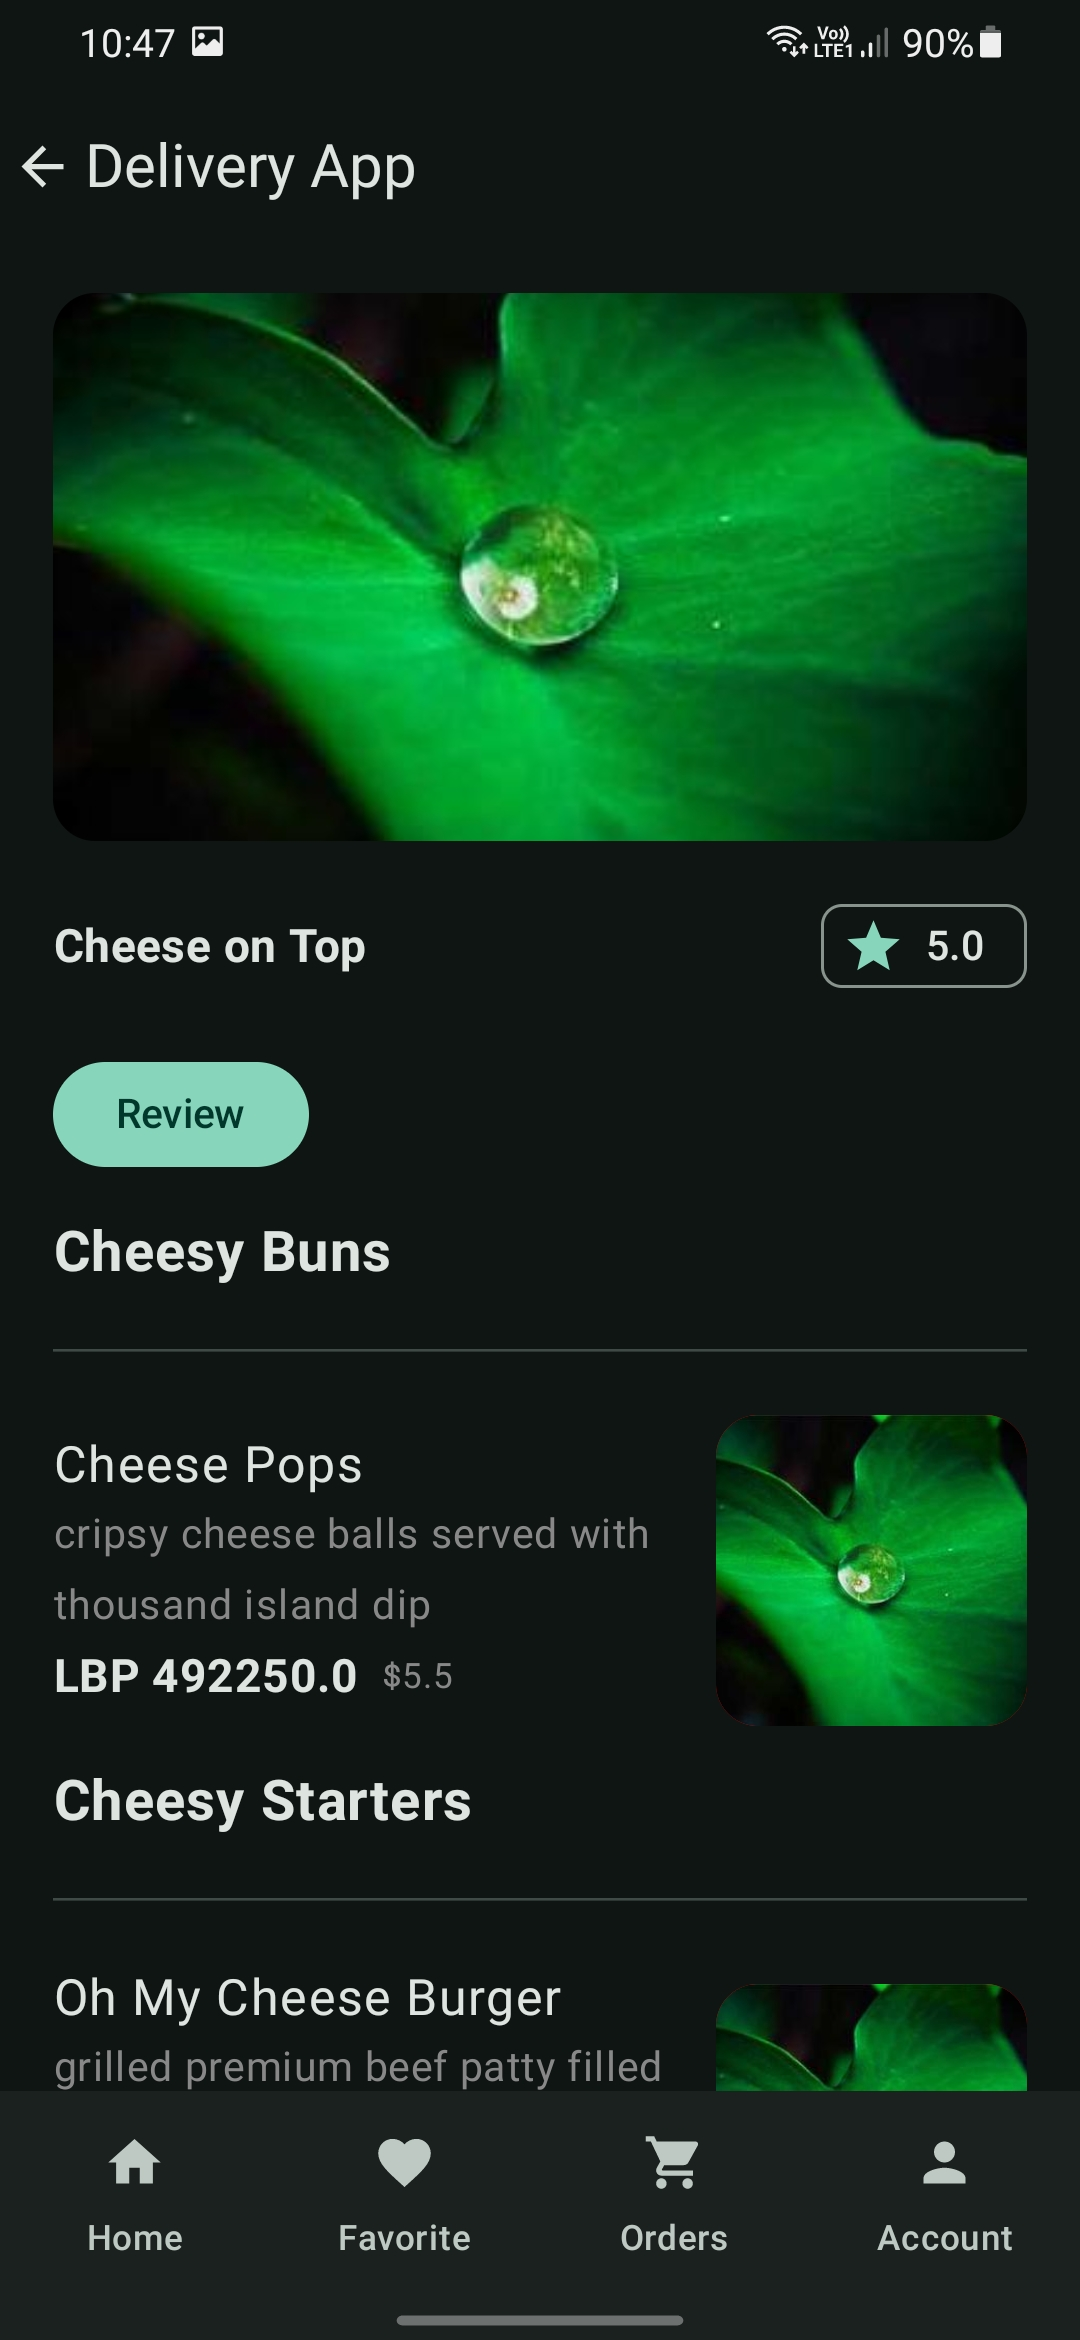
\includegraphics[height=0.7\linewidth]{assets/restaurant.jpg}
    \end{figure}
\end{frame}

\begin{frame}{Features}
    \begin{itemize}
        \item Secure user authentication (JWT).
              \vspace{0.3cm}
        \item Browse and order food from restaurants.
              \vspace{0.3cm}
        \item Mark your favorite restaurants for faster access.
              \vspace{0.3cm}
        \item Submit and view restaurant reviews.
              \vspace{0.3cm}
        \item View order history (past and pending orders).
              \vspace{0.3cm}
        \item Order tracking.
              \vspace{0.3cm}
        \item Rate delivery drivers.
              \vspace{0.3cm}
        \item Manage user profile details.
    \end{itemize}
\end{frame}

\begin{frame}{Technical Implementation}
    \textbf{Architecture:}
    \begin{itemize}
        \item \textbf{Pattern:} MVVM (Model-View-ViewModel).
    \end{itemize}
    \textbf{Technologies:}
    \begin{itemize}
        \item \textbf{Libraries:}
              \begin{itemize}
                  \item Retrofit for API calls.
                  \item Room for local database.
                  \item Jetpack Compose for a declarative UI.
                  \item Google Play Services (GM) to access location data.
                  \item LiveData and ViewModel for UI-related data.
                  \item Osmdroid for map rendering.
                  \item JWTDecode for token authentication.
              \end{itemize}
        \item \textbf{Design Patterns:}
              \begin{itemize}
                  \item Singleton for shared resources.
                  \item Repository for data management.
              \end{itemize}
    \end{itemize}
\end{frame}

\begin{frame}{Challenges and Solutions}
    \begin{tabular}{| p{5cm} | p{5cm} |}
        \hline
        \textbf{Challenge}                                        & \textbf{Solution}                                                             \\
        \hline
        Maintain JWT across sessions                              & Secure storage in SharedPreferences and validation using JWTDecode.           \\
        \hline
        Maintain state across activities                          & Used shared ViewModel instances.                                              \\
        \hline
        Integrate Jetpack Compose with traditional View-based UIs & Clear project structure enabled seamless integration of both UI technologies. \\
        \hline
    \end{tabular}
\end{frame}

\begin{frame}{Future Enhancements}
    \begin{itemize}
        \item Add more information to the user profile.
              \vspace{0.3cm}
        \item Implement advanced order customization options.
              \vspace{0.3cm}
        \item Add support for real-time order tracking.
              \vspace{0.3cm}
        \item Allow restaurant and driver communication.
              \vspace{0.3cm}
        \item Integrate machine learning for personalized recommendations.
    \end{itemize}
\end{frame}

\begin{frame}{Future Enhancements}
    \begin{itemize}
        \item Add rewards, credits, and promo codes.
              \vspace{0.3cm}
        \item Support chat with customer service.
              \vspace{0.3cm}
        \item Enhance UI and transitions between screens.
              \vspace{0.3cm}
        \item Improve the restaurants page with a search bar.
              \vspace{0.3cm}
        \item Add notification and advertising support.
    \end{itemize}
\end{frame}

\begin{frame}{Thank you}
    Repository Link: \texttt{\href{https://github.com/Ghaadyy/delivery-app}{https://github.com/Ghaadyy/delivery-app}}
\end{frame}

\end{document}
